Describes which method has been used in the attempt to classify atlantic right whales from images.

\subsection{Preprocessing}


\subsubsection{Clustering}


\subsubsection{Resizing}


\subsection{Classification Algorithm}
Also known as \emph{Supervised Learning Algorithm}
Discribes which algorithm was used to classify atlantic right whales. Classification Algorithm have one thing in common which is that they require data input to be on a similar data structure.
The overall data structure for Classification is that in can contain 1..n Observations which each has x amount of data points. For a model, the amount of data points for each observation has to be the same. An example as seen in Table \ref{tab:example data} shows how data could look.
If an observation is missing a value it can be set to NA instead. It still has to be present in the structure.

\begin{table}
  \centering
  \caption{Example data}
  \label{tab:example data}
  \begin{tabularx}{\linewidth}{|l|X|X|X|X|} \hline
    obs. & x1 & x2 & x3 & x4 \\ \hline
    1    & 20 & 74 & 84 & 82 \\ \hline
    2    & 52 & 33 & 4  & 36 \\ \hline
    3    & 78 & 55 & 57 & 3  \\ \hline
    4    & 61 & 68 & 65 & 5  \\ \hline
  \end{tabularx}
\end{table}

\subsubsection{Decision Tree}
Decision tree is a classificaion algorithm. A tree structure and binary decisions at each node in order to further limit the amount of possible classes down each path.
At the end of a path, a leaf contains the class to represent that exact path.
When prediction against a decion tree that leaf is given as the returned prediction.

\subsubsection{Random Forest}
Random Forest is an algorithm which is based upon the decision trees and wisdom of the crowd.
Random Forest spawn multiple decision trees, the algorithm for splitting in the decisions tree in random forest does however differs from how it is done in normal decisions trees.
Random Forest use ``feature bagging'' at each node and then decide for the splitting feature on that subset rather than all the features. This ensures that decision trees isn't identical, but offers variaeity.

\subsubsection{Neural Network}
Neural Networks is an algorithm as an attempt to minic how human learns.
Neural Networks do however variate from how neurons and connections works in the brain as it contains a link from each node in layer x to each node in layer x + 1. As seen at Figure \ref{fig:neuralnetwork}, a neural network with only a input layer and a output layer is shown and the connections between the nodes. Each input node in the figure is connected to all the output nodes.

\begin{figure}
  \centering
  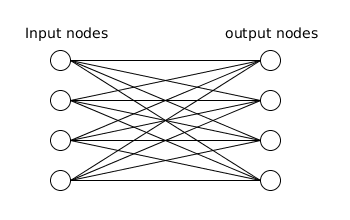
\includegraphics[width=0.7\linewidth]{Images/neuralnetwork}
  \caption{Neural Network with no hidden layers}
  \label{fig:neuralnetwork}
\end{figure}

